% ---
% Reemplaza parte de la sección de resultados en Docs/Technical_Report.tex.
% Entradas que lo respaldan: H-018, H-019, H-031, H-036, H-037, H-038, H-039, H-040, H-041, H-055, D-029, D-033, D-042.
% ---

\subsection{Separabilidad de las representaciones}
\label{sec:separabilidad_representaciones}

% fuente: H-031, H-037; 5a_resumen.csv, 5b_concentracion_kernel.csv
En la evaluación del kernel cuántico de fidelidad a escala nominal ($c = 1$) sobre la submuestra
estratificada de 200 lesiones de entrenamiento por subconjunto, las matrices de similitud resultaron
cercanas a la identidad. En masas, la mediana fuera de la diagonal fue de 0.0022 en C4 (con percentil 95
de 0.011 y 23\,\% de pares con fidelidad inferior a $10^{-3}$) y de 0.000032 en C5 (con 80\,\% de pares
por debajo de $10^{-3}$ y 26\,\% por debajo de $10^{-6}$). En calcificaciones, la mediana fue de 0.0029
en C4 (percentil 95 de 0.014 y 16\,\% bajo $10^{-3}$) y de 0.000031 en C5 (76\,\% bajo $10^{-3}$ y 28\,\%
bajo $10^{-6}$). En contraste, el kernel clásico gaussiano RBF con parámetro $\gamma$ determinado por la
heurística de la mediana registró una mediana fuera de la diagonal de 0.607 en ambos subconjuntos.

% fuente: H-037; X3_comparacion_k8_k12.csv (family «B, embeddings (full train)», k = 12).
% Corregido el 2026-10-19 (auditoría A2-2): 0.056 de 5a_resumen.csv es sobre las 1,696 masas
% (entrenamiento y prueba); sobre el entrenamiento es 0.058, como en la tabla de esta sección.
Sobre todas las lesiones del conjunto de entrenamiento (1\,318 masas y 1\,546 calcificaciones),
la desviación estándar media por dimensión de los valores esperados $\langle Z_i \rangle$ fue de 0.058
en masas y 0.048 en calcificaciones para C4, mientras que en C5 ascendió a 0.180 en masas y 0.178 en
calcificaciones. En C4 las compuertas aplicadas tras la capa inicial de Hadamard son diagonales, por lo
que el término propio en $Z$ añade una variación angular moderada frente a las fases de acoplamiento $ZZ$.
En C5, la rotación no diagonal en el eje $Y$ modifica directamente las amplitudes antes de la acción de
los términos $ZZ$, dispersando los valores esperados locales pero acentuando la ortogonalidad mutua en el
espacio de estados cuánticos y concentrando la fidelidad unas setenta veces más que en C4 \cite{Thanasilp2024}.

% fuente: H-018, H-019; B3_concentracion_embedding.csv
Esta concentración del \textit{embedding} reproduce el comportamiento caracterizado en el estudio B3
sobre la dispersión de los valores esperados $\langle Z_i \rangle$ (evaluada sobre 100 entradas y 10 sorteos de $\boldsymbol\theta$
con cálculo analítico exacto tras corregir la inyección de ruido en la referencia). Dicho análisis evidenció tres
patrones fundamentales: en primer lugar, la concentración con el número de qubits es sistemática, reduciéndose la dispersión media
a \texttt{reps} = 1 de $0.0837 \pm 0.0131$ con $k = 8$ a $0.0417 \pm 0.0068$ con $k = 12$ y a $0.0363 \pm 0.0090$ con $k = 16$,
comportamiento característico del crecimiento exponencial del espacio de Hilbert y precursor de las mesetas áridas (\textit{barren plateaus}).
En segundo lugar, la concentración con la profundidad del circuito no es monótona en el rango analizado: para $k = 12$, la dispersión
se incrementa en un 30\,\% al pasar de \texttt{reps} = 1 a \texttt{reps} = 2 ($0.0417 \pm 0.0068$ frente a $0.0544 \pm 0.0036$),
descendiendo a $0.0305 \pm 0.0044$ con \texttt{reps} = 3. En tercer lugar, la variabilidad entre distintos sorteos del vector $\boldsymbol\theta$
colapsa con la profundidad: a $k = 16$, la desviación entre sorteos se reduce de 0.0090 a 0.0043 y finalmente a 0.0023, reflejando
una pérdida progresiva de sensibilidad respecto a los parámetros del circuito que es indicativa del régimen de meseta árida.

\begin{figure}[htbp]
\centering
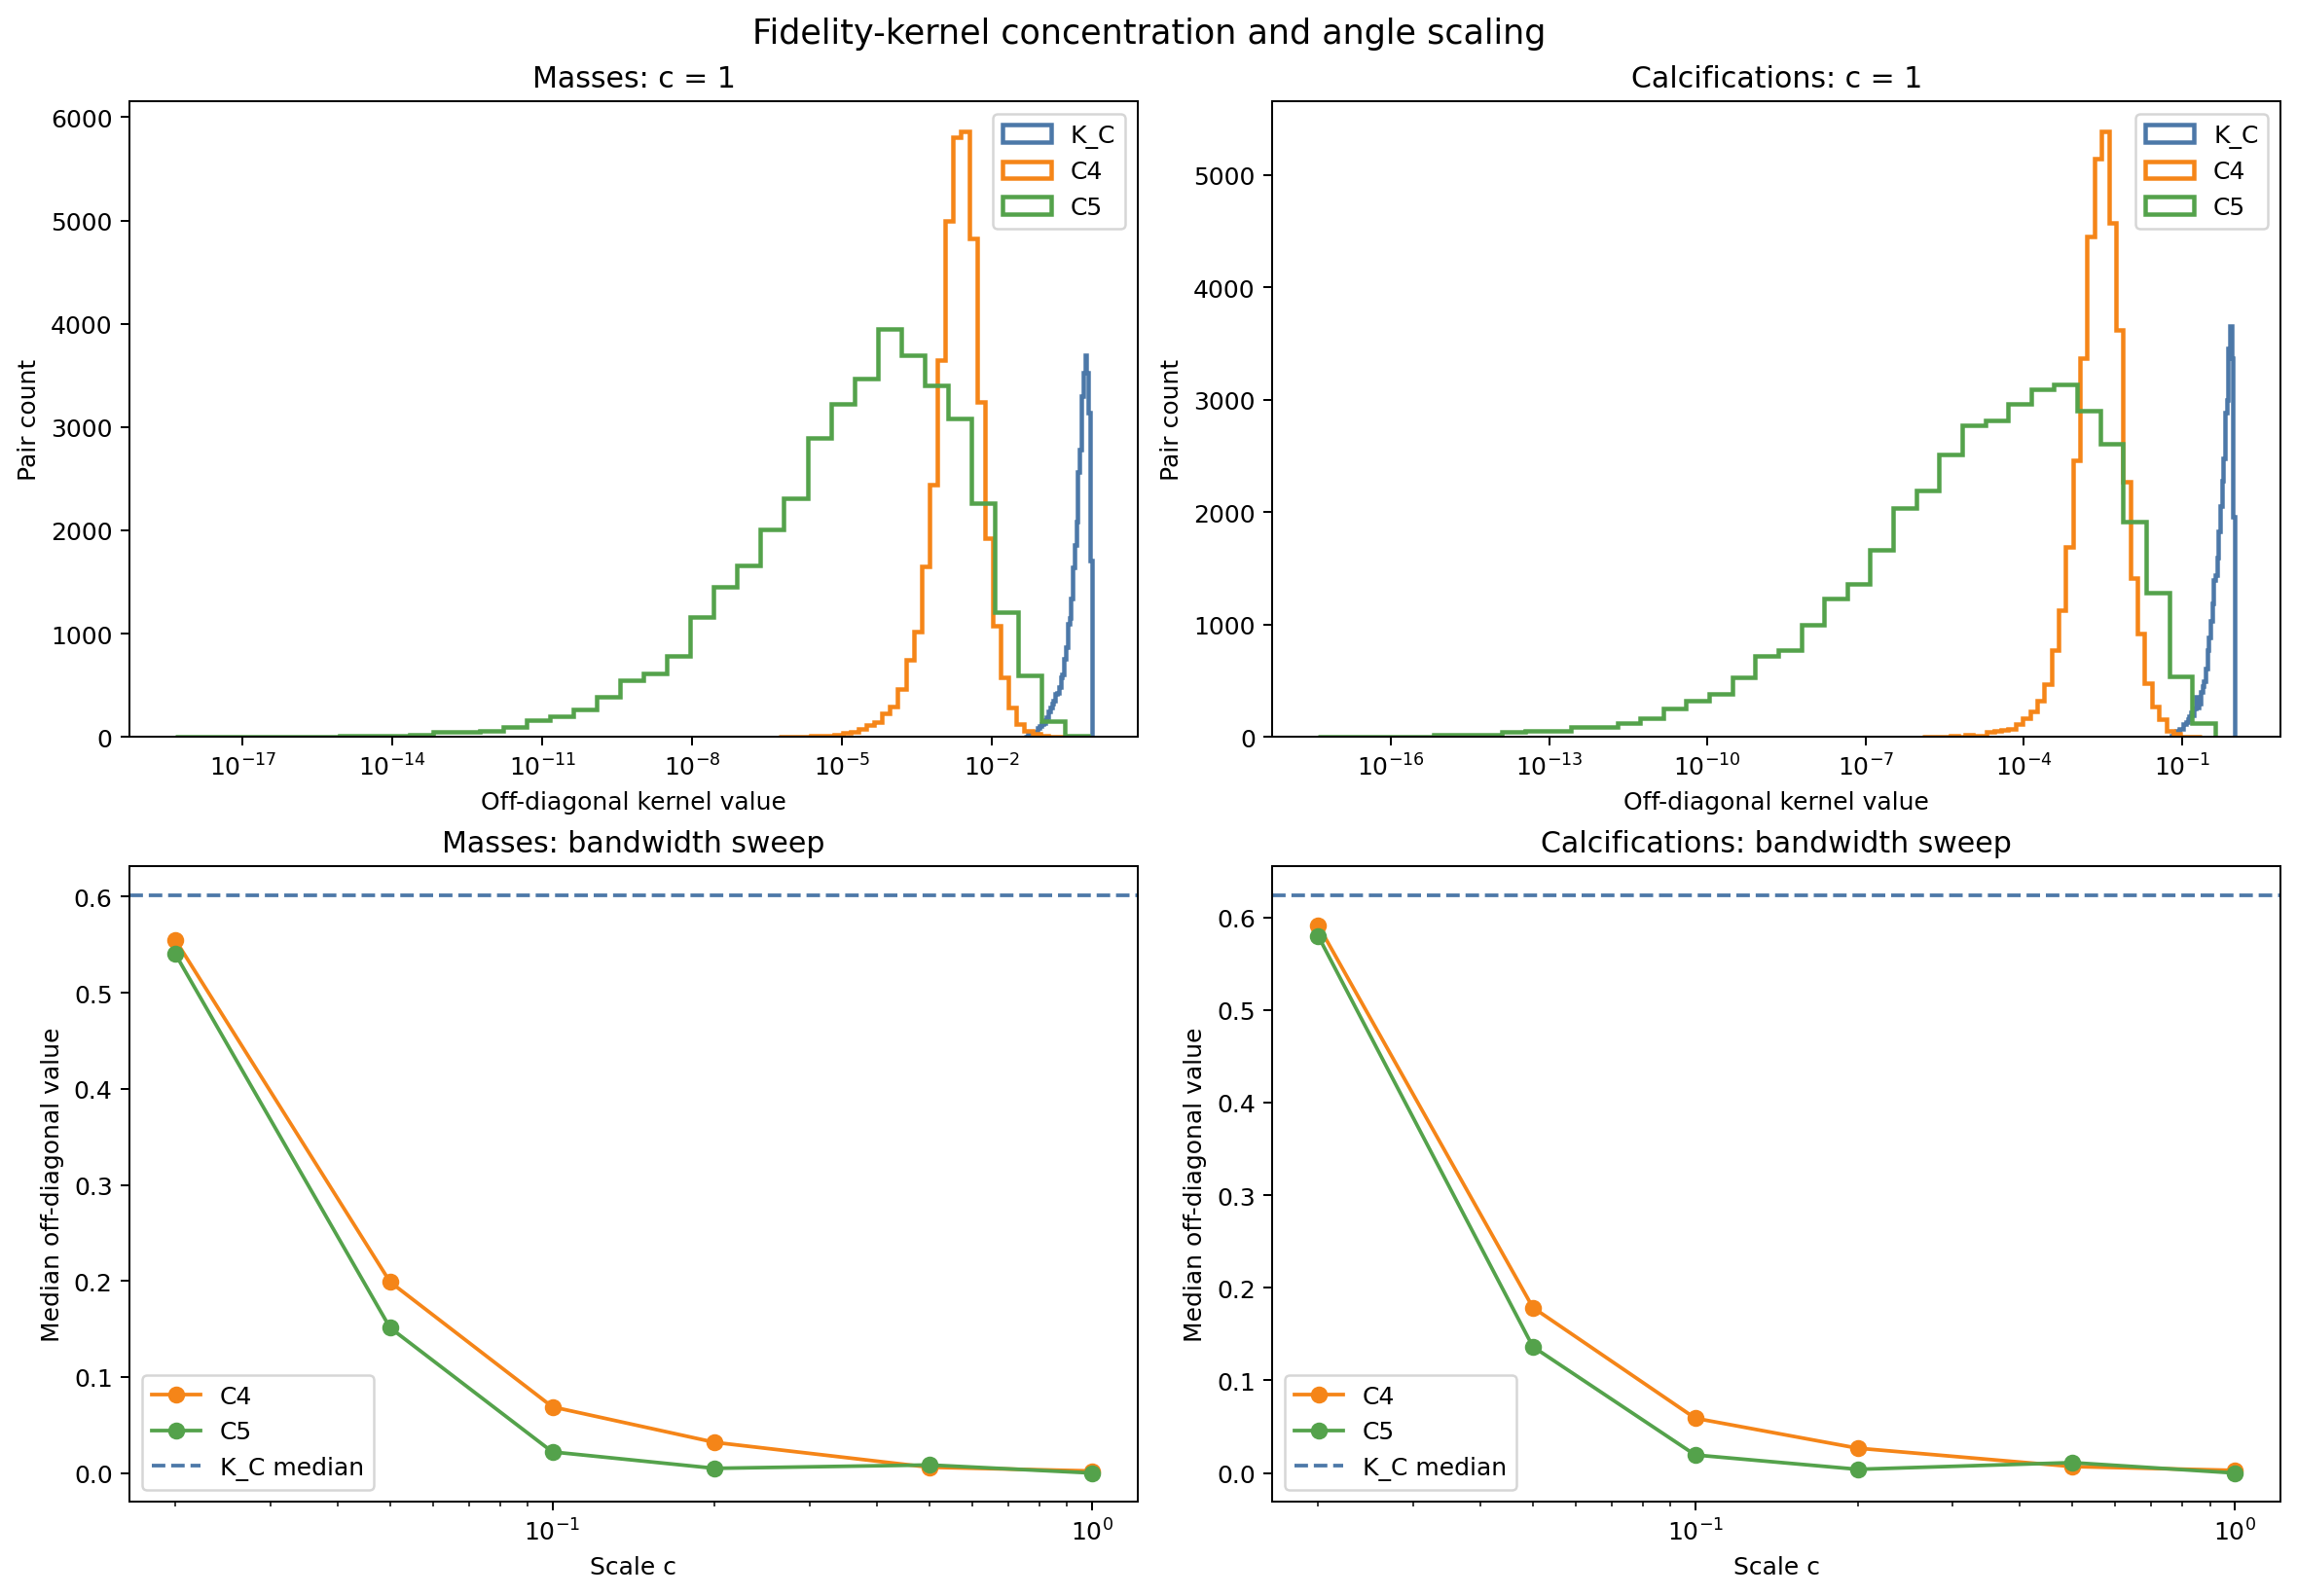
\includegraphics[width=\textwidth]{Figures/M5_kernel_concentration.png}
% fuente: H-031, H-037; 5b_concentracion_kernel.csv
\caption{Distribución de los valores fuera de la diagonal en las matrices de kernel cuántico para C4 y C5 frente al kernel clásico RBF.}
\label{fig:m5_kernel_concentration}
\end{figure}

% fuente: H-038, H-039; 6_alineamiento_kernel.csv, 6_dimension_efectiva.csv, 6_diferencia_geometrica_resumen.csv
Los resultados de separabilidad formal en la familia de kernels se resumen en la
Tabla~\ref{tab:m6_kernels}, calculados sobre la submuestra de entrenamiento con $c = 1$.

% fuente: H-038, H-039; 6_alineamiento_kernel.csv, 6_dimension_efectiva.csv, 6_diferencia_geometrica_resumen.csv
% Generado por Code/tools/tablas_latex.py desde 6_alineamiento_kernel.csv, 6_dimension_efectiva.csv y 6_diferencia_geometrica_resumen.csv. No editar a mano: volver a correr el script.
\begin{table}[H]
\centering
\small
\caption{Separabilidad en la familia de kernels (M6), $c = 1$, 200 lesiones de entrenamiento por subconjunto.}
\label{tab:m6_kernels}
\begin{adjustbox}{max width=\linewidth}
\begin{tabular}{l r r r r r}
\toprule
Kernel & KTA centrada & Exceso sobre permutación & $p$ & $d_{\mathrm{eff}}$ (de 200) & $g$ regularizada \\
\midrule
\multicolumn{6}{l}{\textit{Masas}} \\
\quad RBF (clásico) & 0.059 & 0.049 & $<$0.001 & 2.8 & — \\
\quad C4, ZZ & 0.073 & 0.003 & 0.002 & 184.0 & 1.433 \\
\quad C5, Y--ZZ & 0.075 & 0.005 & 0.003 & 171.3 & 1.511 \\
\multicolumn{6}{l}{\textit{Calcificaciones}} \\
\quad RBF (clásico) & 0.161 & 0.151 & $<$0.001 & 2.6 & — \\
\quad C4, ZZ & 0.077 & 0.006 & $<$0.001 & 187.7 & 1.400 \\
\quad C5, Y--ZZ & 0.075 & 0.007 & 0.003 & 167.6 & 1.701 \\
\bottomrule
\end{tabular}
\end{adjustbox}
\par\smallskip
\parbox{0.95\linewidth}{\footnotesize El exceso es la KTA centrada menos la media de 1{,}000 permutaciones de etiquetas; $p$ es unilateral. $g$ es el mínimo de la \textit{geometric difference} regularizada sobre la batería de kernels clásicos del Apéndice L.3 de Huang et al.\; $\sqrt{N} \approx 14$.}
\end{table}


% fuente: H-038, H-039; 6_alineamiento_kernel.csv
El exceso de alineamiento centrado (\textit{kernel-target alignment}, KTA) sobre la media de 1\,000
permutaciones de etiquetas fue en masas de 0.049 ($p < 0.001$) para el kernel clásico RBF, frente a 0.003
($p = 0.002$) en C4 y 0.005 ($p = 0.003$) en C5. En calcificaciones, el exceso del kernel RBF fue de 0.151
($p < 0.001$), frente a 0.006 ($p < 0.001$) en C4 y 0.007 ($p = 0.003$) en C5. Aunque el exceso en los
kernels cuánticos resultó estadísticamente significativo, representó únicamente entre el 4\,\% y el 10\,\%
del exceso clásico. Los valores absolutos de KTA centrada en C4 y C5 ($0.073$ a $0.077$) se encuentran
acotados por el valor base de $1/\sqrt{N-1} \approx 0.071$ inherente a matrices cercanas a la identidad
para muestras de $N = 200$ \cite{Cortes2012}.

% fuente: H-038, H-039; 6_dimension_efectiva.csv
La dimensión efectiva normalizada ($d_{\mathrm{eff}}$ de 200) arrojó 2.8 en masas y 2.6 en
calcificaciones para el kernel clásico RBF. Para los kernels cuánticos, los valores fueron de 184.0 en C4
y 171.3 en C5 para masas, y de 187.7 en C4 y 167.6 en C5 para calcificaciones. Las representaciones
cuánticas ocupan casi la totalidad de las dimensiones del espacio disponible ($d_{\mathrm{eff}} \approx N$),
régimen en el cual las cotas teóricas de error de generalización derivadas por Huang et al. \cite{huang2021power}
se aproximan a su valor máximo al escalar con $\sqrt{\min(d_{\mathrm{eff}}, \operatorname{Tr}(O^2))/N}$.

% fuente: H-038, H-039; 6_diferencia_geometrica_resumen.csv
En la métrica de diferencia geométrica regularizada frente a la batería de kernels clásicos,
los valores mínimos obtenidos fueron $g = 1.433$ en C4 y $1.511$ en C5 para masas, y $g = 1.400$ en C4
y $1.701$ en C5 para calcificaciones. En comparación con la cota de referencia $\sqrt{N} \approx 14.1$,
se cumple de forma consistente la condición $g \ll \sqrt{N}$, bajo la cual el marco teórico de Huang et al.
\cite{huang2021power} indica que los modelos clásicos pueden igualar o mejorar el desempeño del modelo cuántico
con cualquier vector de etiquetas. En la batería clásica extendida con gaussianos estrechos, el valor mínimo
se reduce a 1.31 en C4 y 1.48 en C5 para masas, y a 1.38 en C4 y 1.70 en C5 para calcificaciones. Por el contrario,
el cálculo de $g$ sin regularizar genera valores entre 306 y 388 (próximos a la cota teórica de $K_Q = I$,
$1/\sqrt{\lambda_{\min}(K_C)} \approx 410$), producto del condicionamiento numérico de la matriz clásica invertida.

\begin{figure}[htbp]
\centering
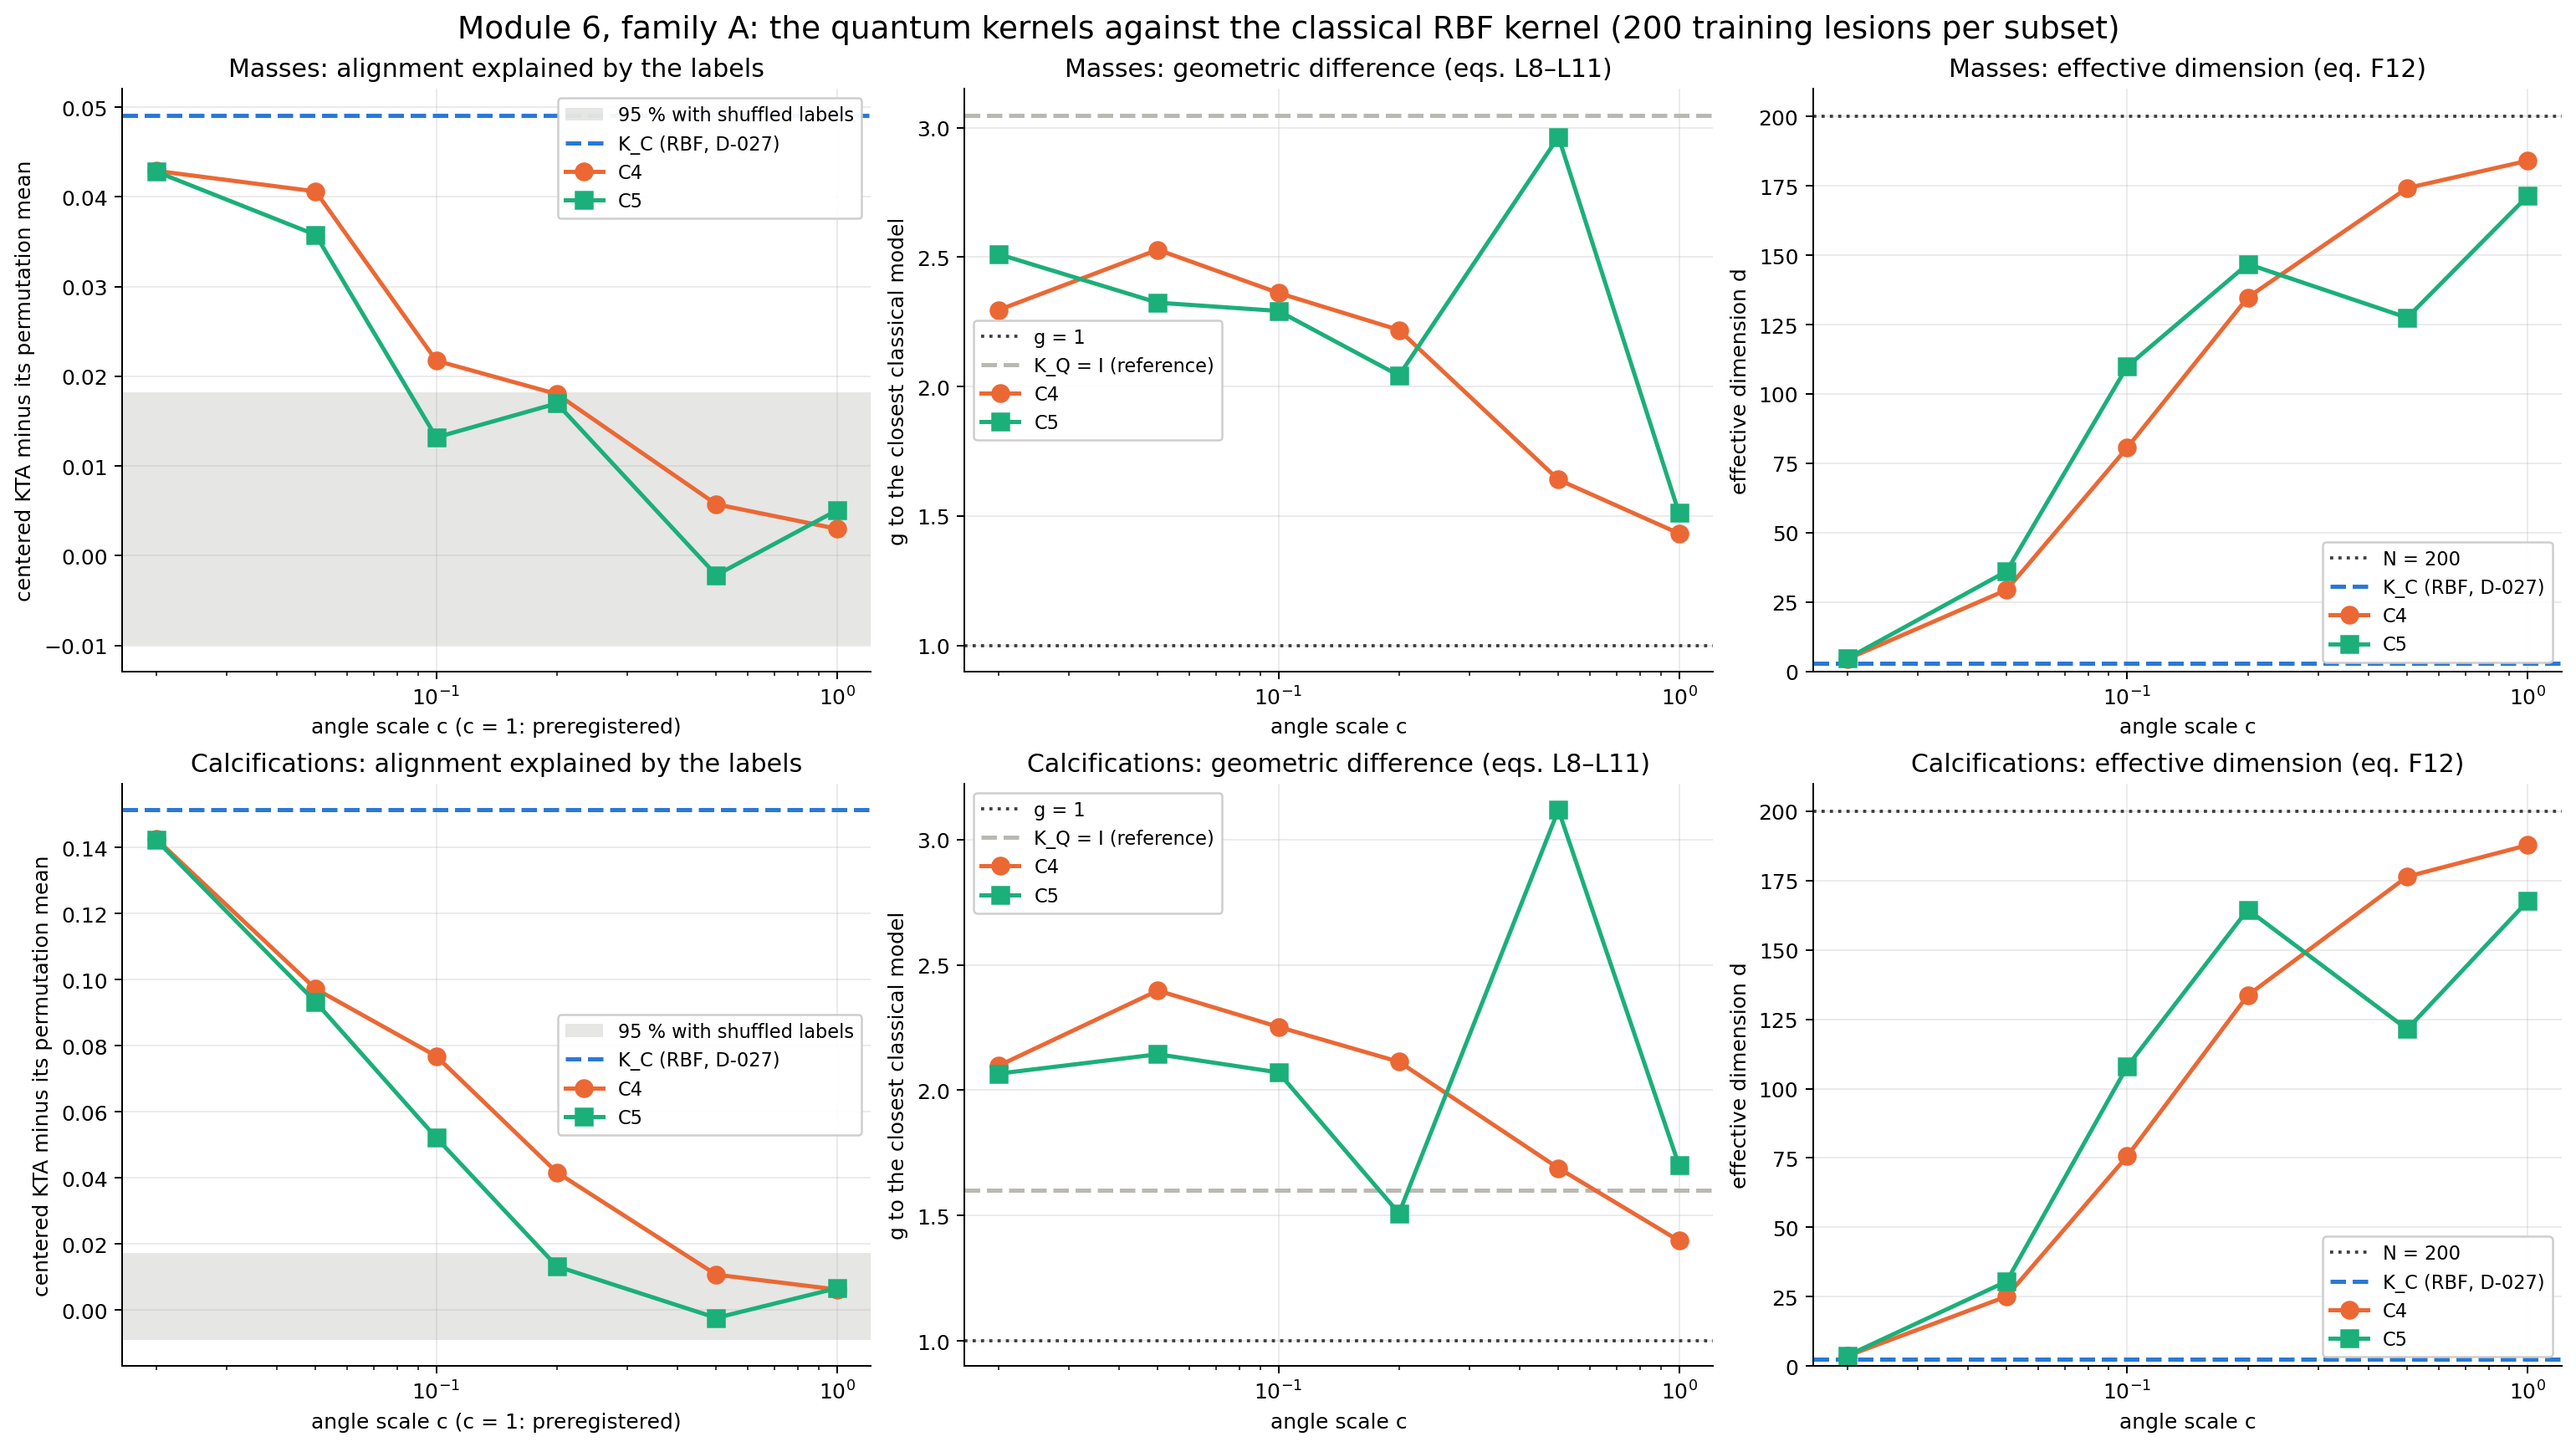
\includegraphics[width=\textwidth]{Figures/M6_kernel_metrics.png}
% fuente: H-038, H-039; 6_alineamiento_kernel.csv, 6_dimension_efectiva.csv
\caption{Métricas de separabilidad en la familia de kernels: alineamiento KTA y dimensión efectiva normalizada.}
\label{fig:m6_kernel_metrics}
\end{figure}

\begin{figure}[htbp]
\centering
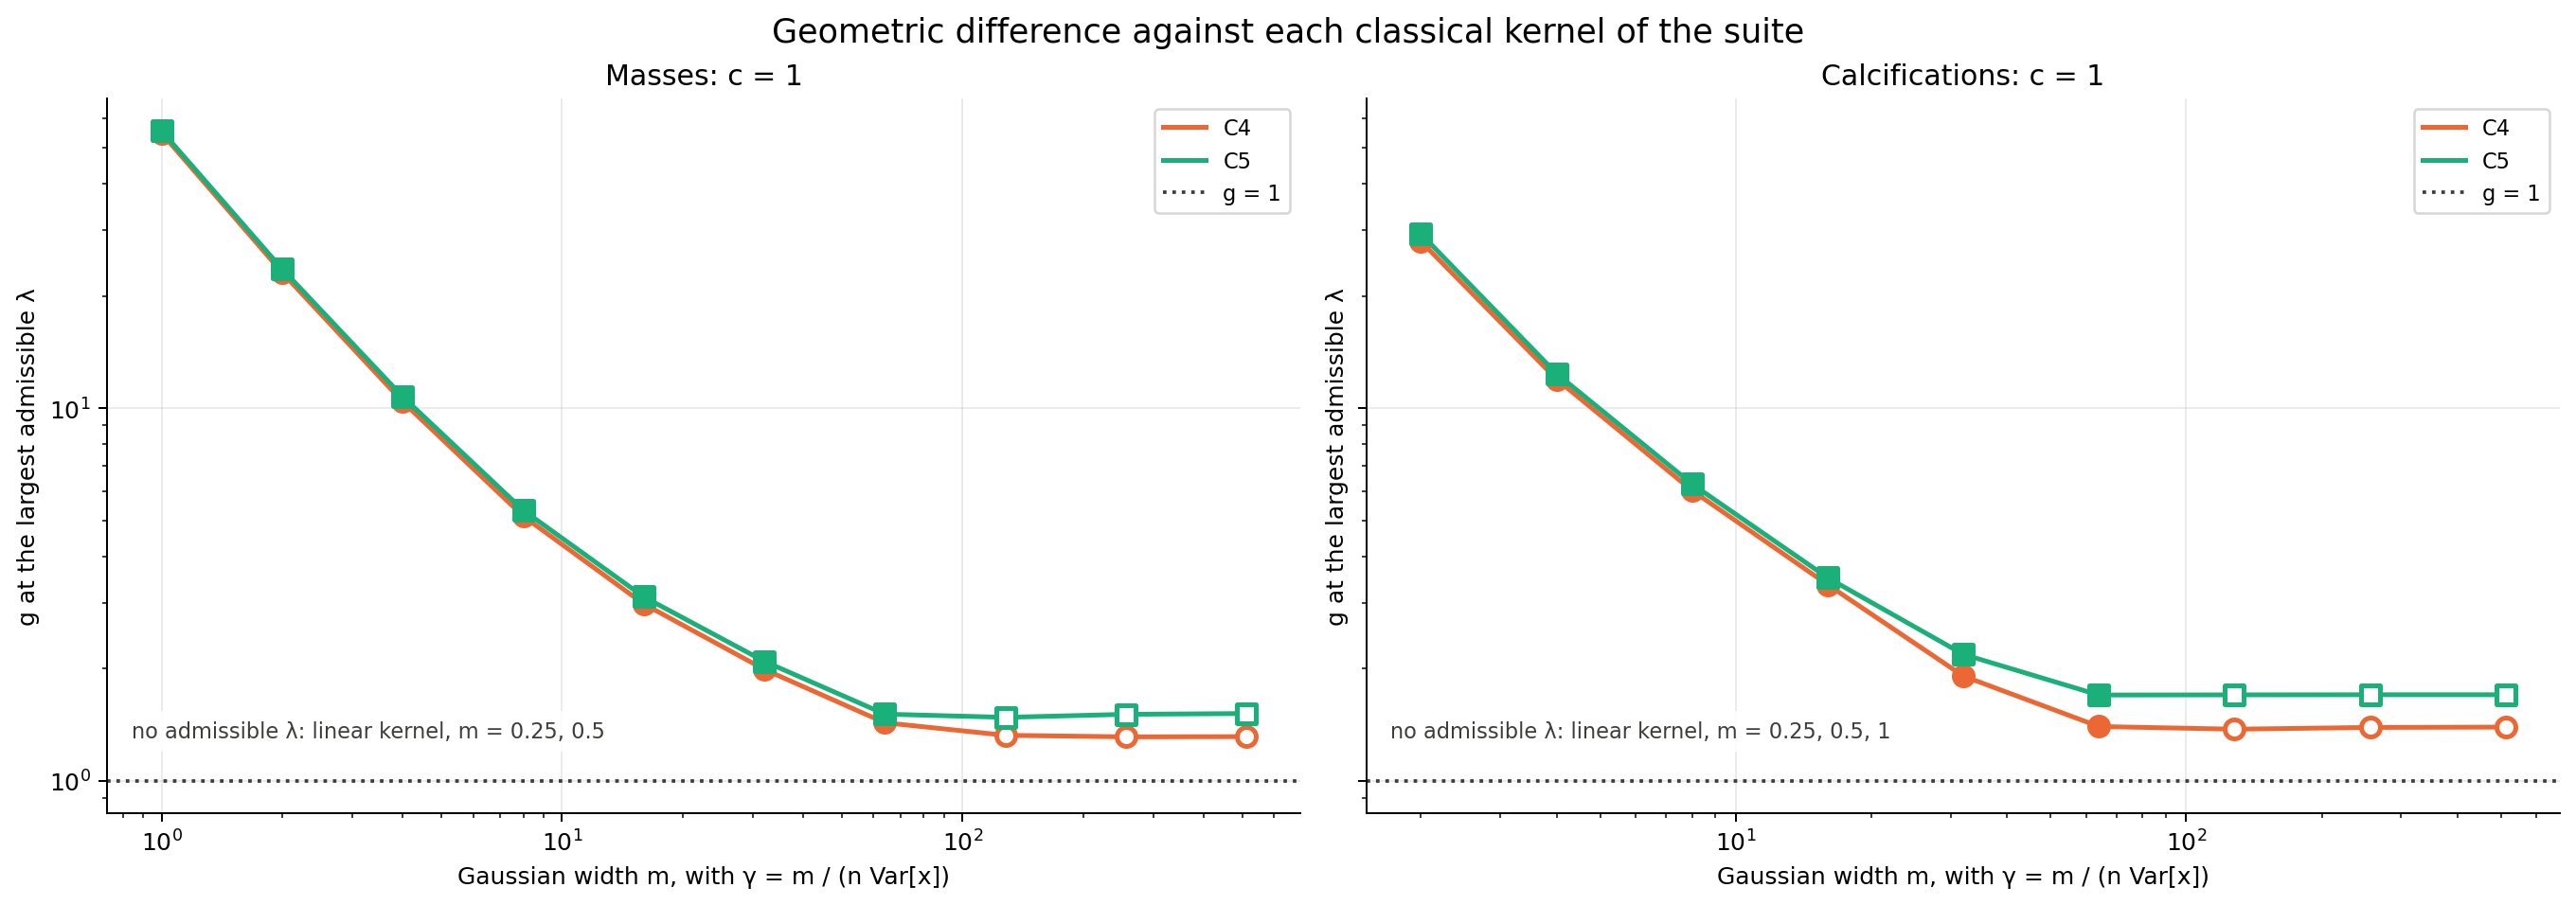
\includegraphics[width=\textwidth]{Figures/M6_geometric_difference.png}
% fuente: H-038, H-039; 6_diferencia_geometrica_resumen.csv
\caption{Diferencia geométrica regularizada $g$ respecto a la batería de modelos clásicos frente al límite $\sqrt{N}$.}
\label{fig:m6_geometric_difference}
\end{figure}

% fuente: H-040; 6_metricas_embedding.csv
La separabilidad sobre las representaciones vectoriales generadas por los cinco esquemas metodológicos
se presenta en la Tabla~\ref{tab:m6_embeddings}.

% fuente: H-040; 6_metricas_embedding.csv
% Generado por Code/tools/tablas_latex.py desde 6_metricas_embedding.csv. No editar a mano: volver a correr el script.
\begin{table}[H]
\centering
\small
\caption{Separabilidad en la familia de embeddings (M6): 200 lesiones de entrenamiento por subconjunto.}
\label{tab:m6_embeddings}
\begin{adjustbox}{max width=\linewidth}
\begin{tabular}{l r r r}
\toprule
Condición & Davies--Bouldin $\downarrow$ & Fisher $J$ $\uparrow$ & KTA lineal $\uparrow$ \\
\midrule
\multicolumn{4}{l}{\textit{Masas}} \\
\quad C1 & 4.301 & 0.669 & 0.070 \\
\quad C2 & 4.301 & 0.669 & 0.070 \\
\quad C3 & 5.564 & 0.781 & 0.059 \\
\quad C4 & 5.898 & 0.449 & 0.041 \\
\quad C5 & 13.346 & 0.668 & 0.012 \\
\multicolumn{4}{l}{\textit{Calcificaciones}} \\
\quad C1 & 2.387 & 1.284 & 0.181 \\
\quad C2 & 2.387 & 1.284 & 0.181 \\
\quad C3 & 2.995 & 1.390 & 0.161 \\
\quad C4 & 6.890 & 0.399 & 0.031 \\
\quad C5 & 6.247 & 0.753 & 0.041 \\
\bottomrule
\end{tabular}
\end{adjustbox}
\par\smallskip
\parbox{0.95\linewidth}{\footnotesize Fisher $J = \Delta\mu^\top S_W^{-1} \Delta\mu$, con la covarianza intraclase combinada. C1 y C2 coinciden por construcción.}
\end{table}


% fuente: H-040; 6_metricas_embedding.csv
En la submuestra de 200 lesiones, las tres representaciones clásicas (C1, C2 y C3) superaron a las
cuánticas (C4 y C5) en todas las métricas evaluadas. En masas, el índice de Davies--Bouldin fue de 4.301 en C1
y C2 frente a 5.898 en C4 y 13.346 en C5 ($p = 0.41$); la razón de Fisher $J$ fue de 0.669 en C1 y C2 (y 0.781 en C3)
frente a 0.449 en C4 ($p = 0.05$) y 0.668 en C5; y el alineamiento lineal fue de 0.070 en C1 y C2 frente a 0.041 en C4
y 0.012 en C5 ($p = 0.41$). En calcificaciones, Davies--Bouldin fue de 2.387 en C1 y C2 frente a 6.890 en C4 y 6.247
en C5; Fisher $J$ fue de 1.284 en C1 y C2 (y 1.390 en C3) frente a 0.399 en C4 ($p = 0.15$) y 0.753 en C5; y el
alineamiento lineal fue de 0.181 en C1 y C2 frente a 0.031 en C4 y 0.041 en C5. Las métricas de C1 y C2 coincidieron
con discrepancias numéricas del orden del límite de precisión ($< 10^{-14}$), lo cual concuerda con la invarianza
teórica de las distancias y dispersiones ante rotaciones ortogonales bajo la condición de control nulo.
Al evaluar la razón de Fisher sobre la totalidad del conjunto de entrenamiento, la ventaja clásica se mantuvo:
C1 obtuvo 0.45 en masas y 1.06 en calcificaciones, frente a 0.13 y 0.42 en C4, y 0.21 y 0.31 en C5.

\begin{figure}[htbp]
\centering
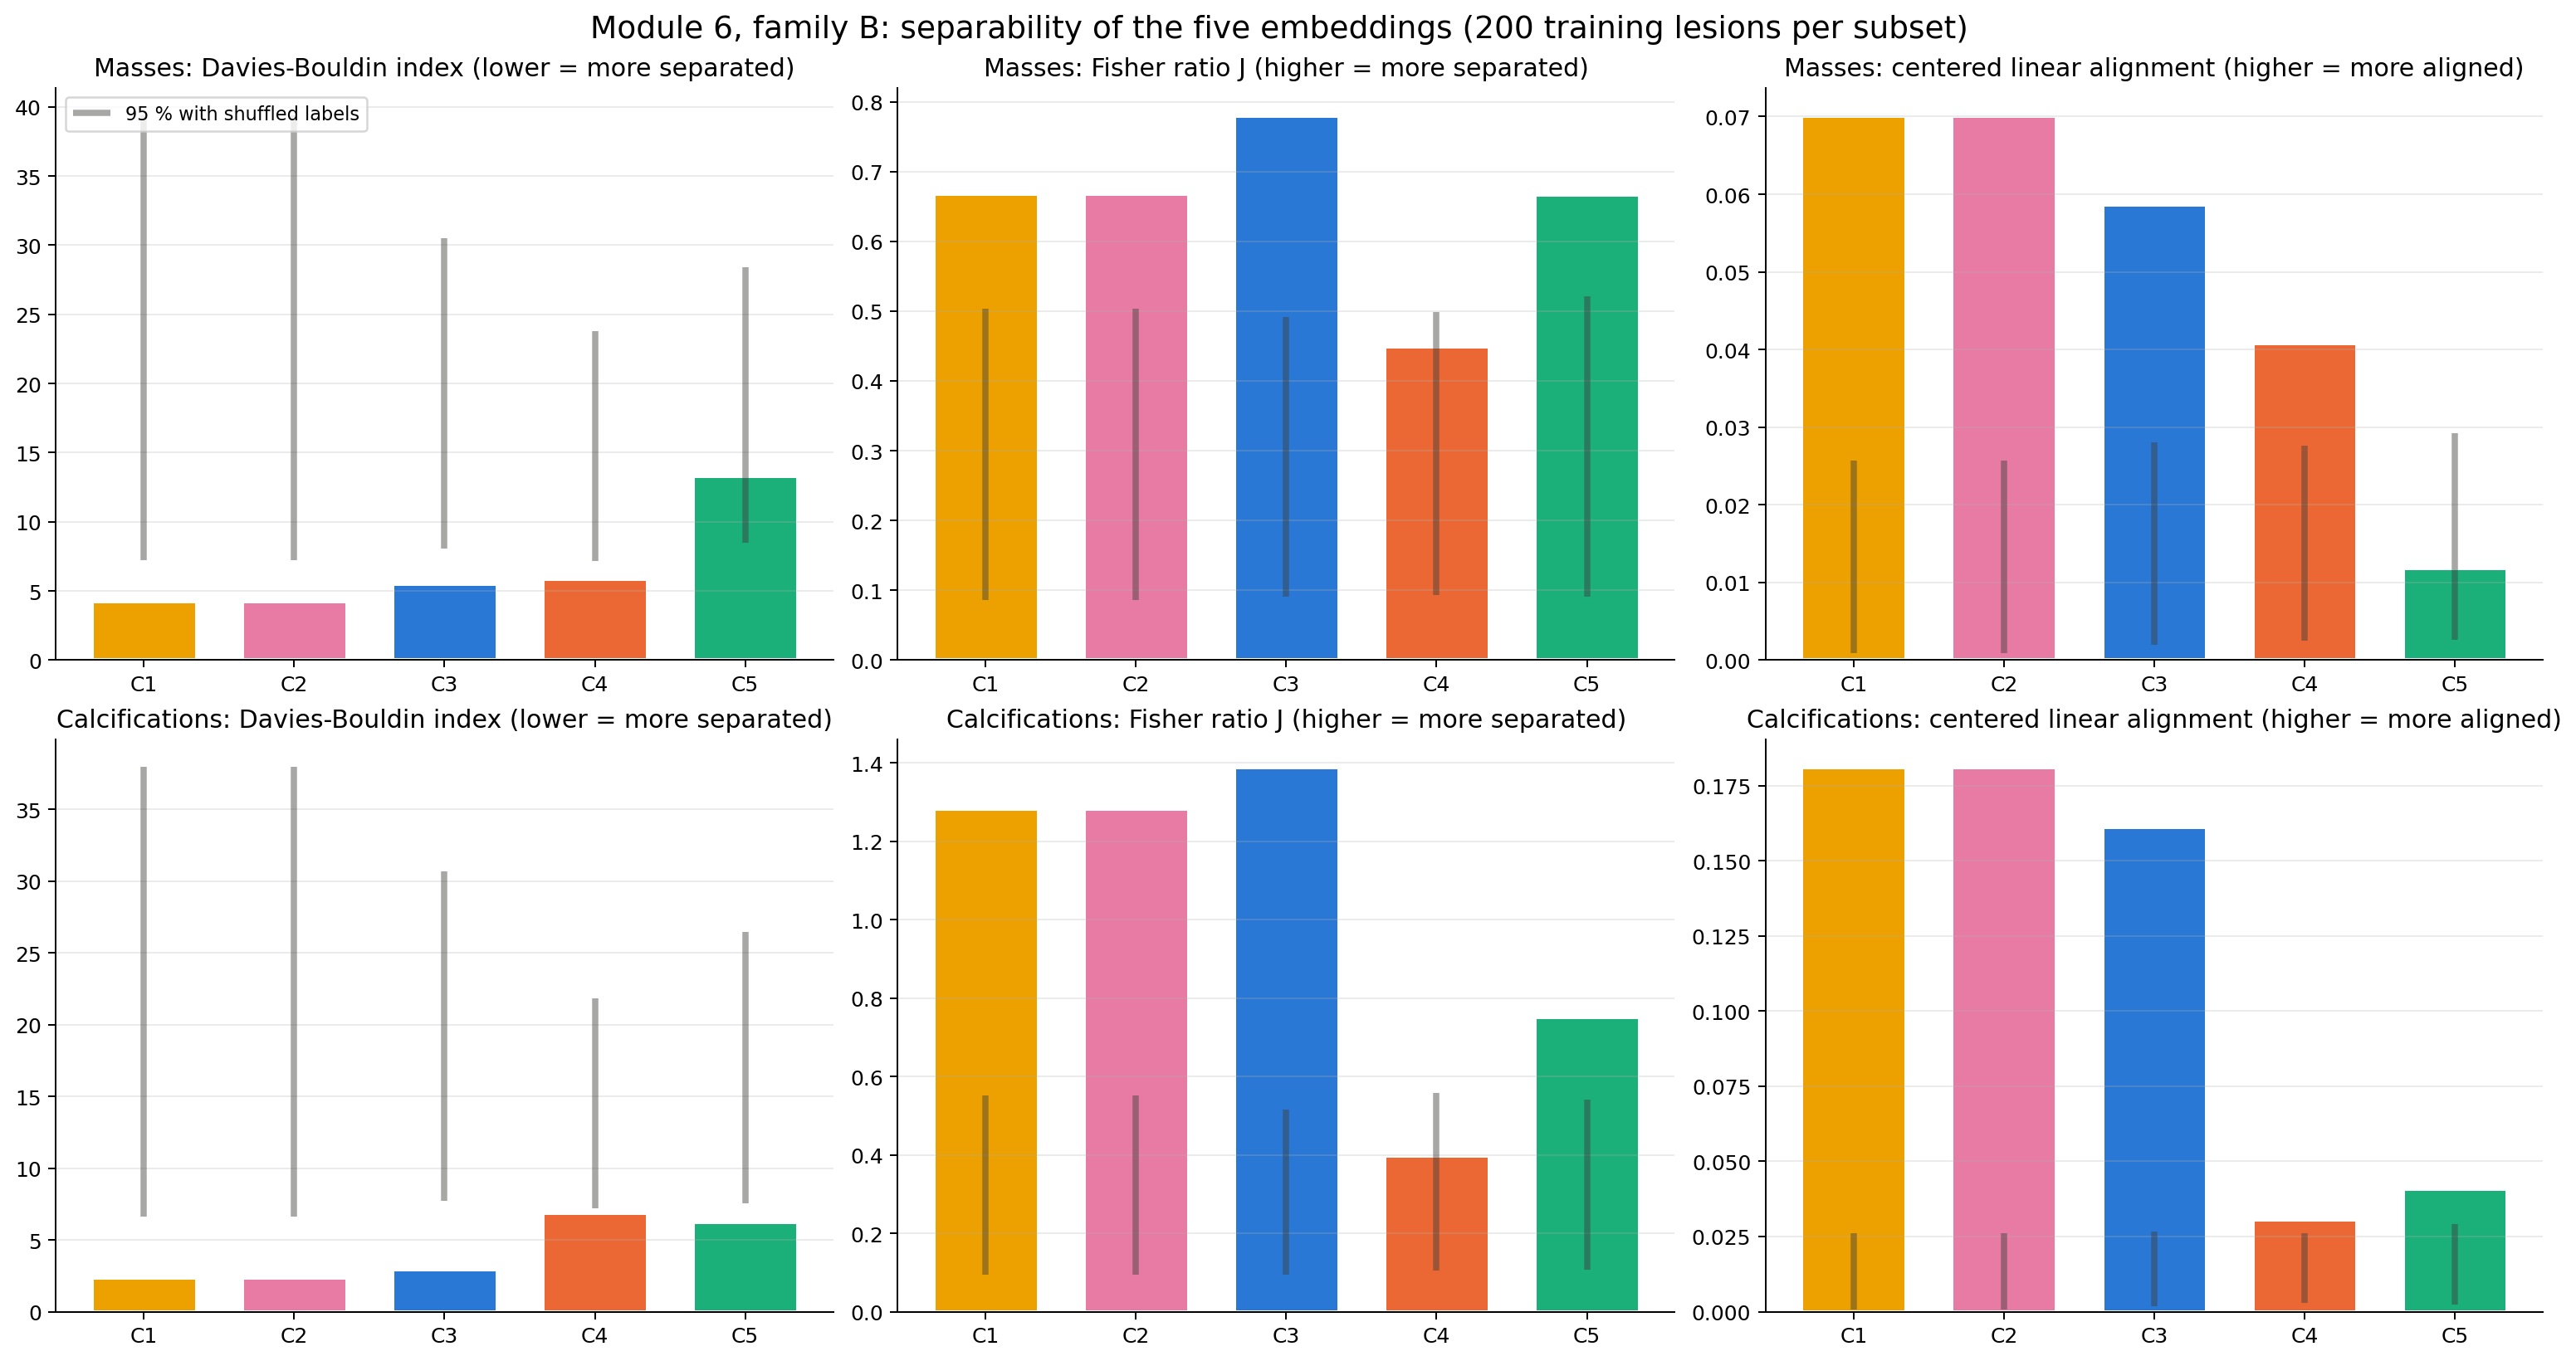
\includegraphics[width=\textwidth]{Figures/M6_embedding_metrics.png}
% fuente: H-040; 6_metricas_embedding.csv
\caption{Métricas de separabilidad sobre las representaciones vectoriales: índice de Davies--Bouldin, razón de Fisher y alineamiento lineal.}
\label{fig:m6_embedding_metrics}
\end{figure}

\begin{figure}[htbp]
\centering
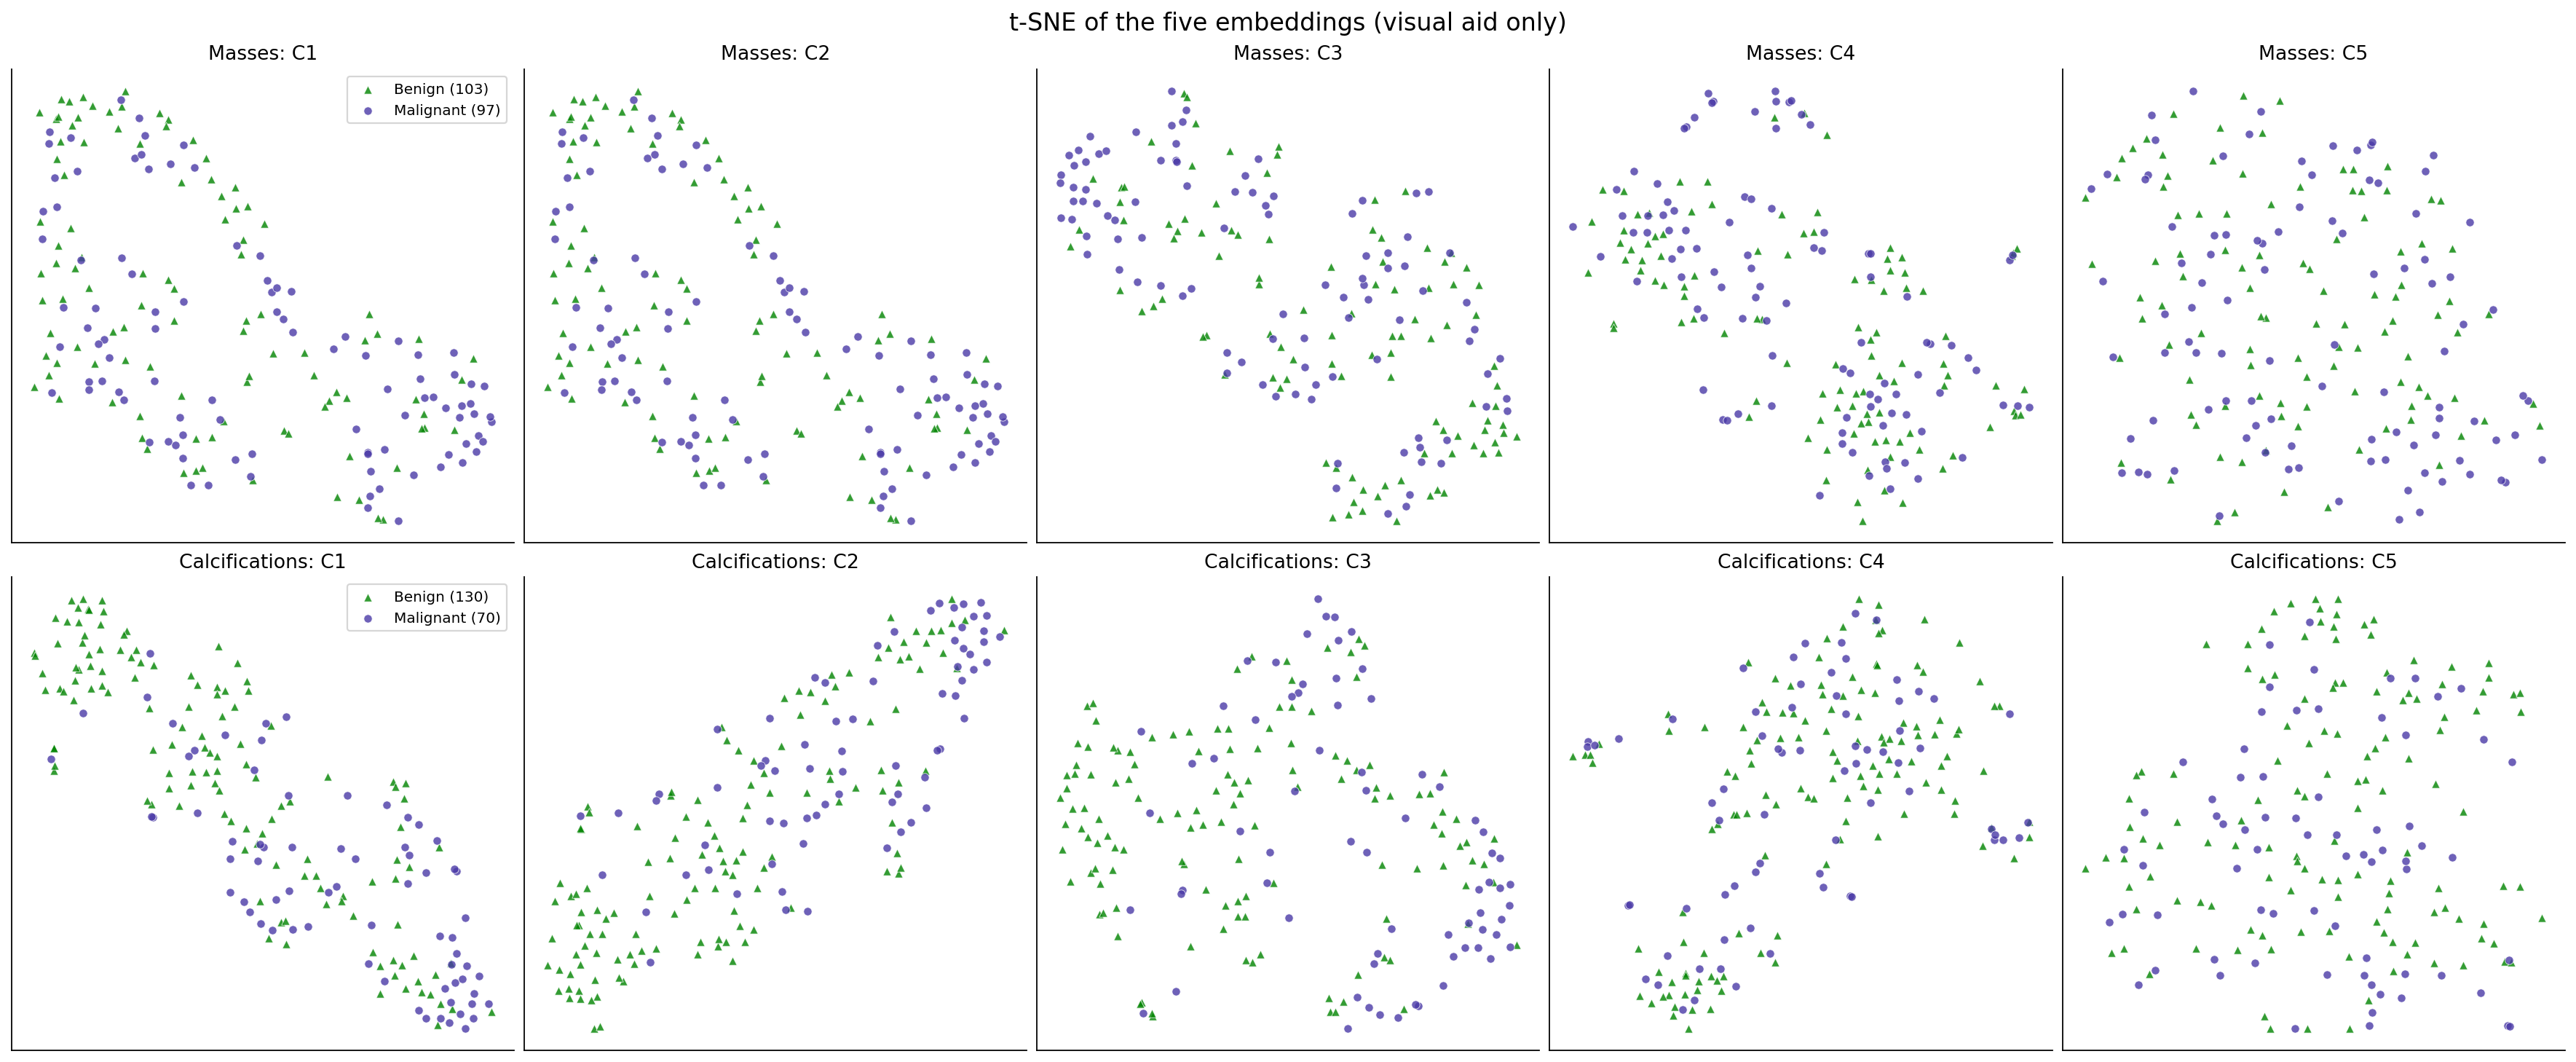
\includegraphics[width=\textwidth]{Figures/M6_tsne.png}
% fuente: H-040; 6_metricas_embedding.csv
\caption{Proyecciones bidimensionales mediante t-SNE para las representaciones generadas en las cinco condiciones.}
\label{fig:m6_tsne}
\end{figure}

% fuente: H-055, D-042; X9_resumen_familia_a.csv, X9_orden_familia_b.csv, X9_familia_a.csv
Para descartar que estas conclusiones dependan de la submuestra, las métricas a $c = 1$ se repitieron
sobre otras 19 submuestras estratificadas de 200 lesiones de entrenamiento y sobre la totalidad del
conjunto de entrenamiento, sin usar el conjunto de prueba (Figura~\ref{fig:x9_sample_size}). En las
20 submuestras de ambos subconjuntos, el kernel RBF conservó un exceso de KTA mayor que el de los dos
kernels cuánticos, sin traslape de rangos: el menor exceso clásico, 0.019 en masas y 0.055 en
calcificaciones, superó al mayor exceso cuántico, 0.011 y 0.014. La diferencia geométrica mínima se
mantuvo entre 1.31 y 2.87, a lo sumo 0.20 veces $\sqrt{N}$, y la dimensión efectiva de C4 y C5, entre
0.82 y 0.95 veces $N$. En las representaciones vectoriales, la mejor condición clásica (C1 o C3) superó
a las dos cuánticas en las 20 submuestras y en las tres métricas. Sobre todo el entrenamiento
(1\,318 masas y 1\,546 calcificaciones), el exceso de KTA fue de 0.055 para el RBF frente a 0.006 (C4)
y 0.009 (C5) en masas, y de 0.148 frente a 0.018 y 0.020 en calcificaciones, con $p = 0.001$ en todos
los casos; $g$ se ubicó entre 2.95 y 3.25, frente a $\sqrt{N}$ de 36.3 y 39.3. El exceso cuántico
crece con $N$ porque en un kernel concentrado la señal de clase reside en los $N(N-1)$ pares fuera de
la diagonal, cada uno con un traslape mínimo; por ello los valores de alineamiento, $g$ y dimensión
efectiva solo se comparan entre condiciones con el mismo $N$. Dos aspectos sí dependen de la muestra:
la significancia de los efectos más pequeños, pues C5 en masas llegó a $p = 0.24$ en alguna submuestra,
y el orden entre C4 y C5, que cambia con la métrica y con la submuestra.

\begin{figure}[htbp]
\centering
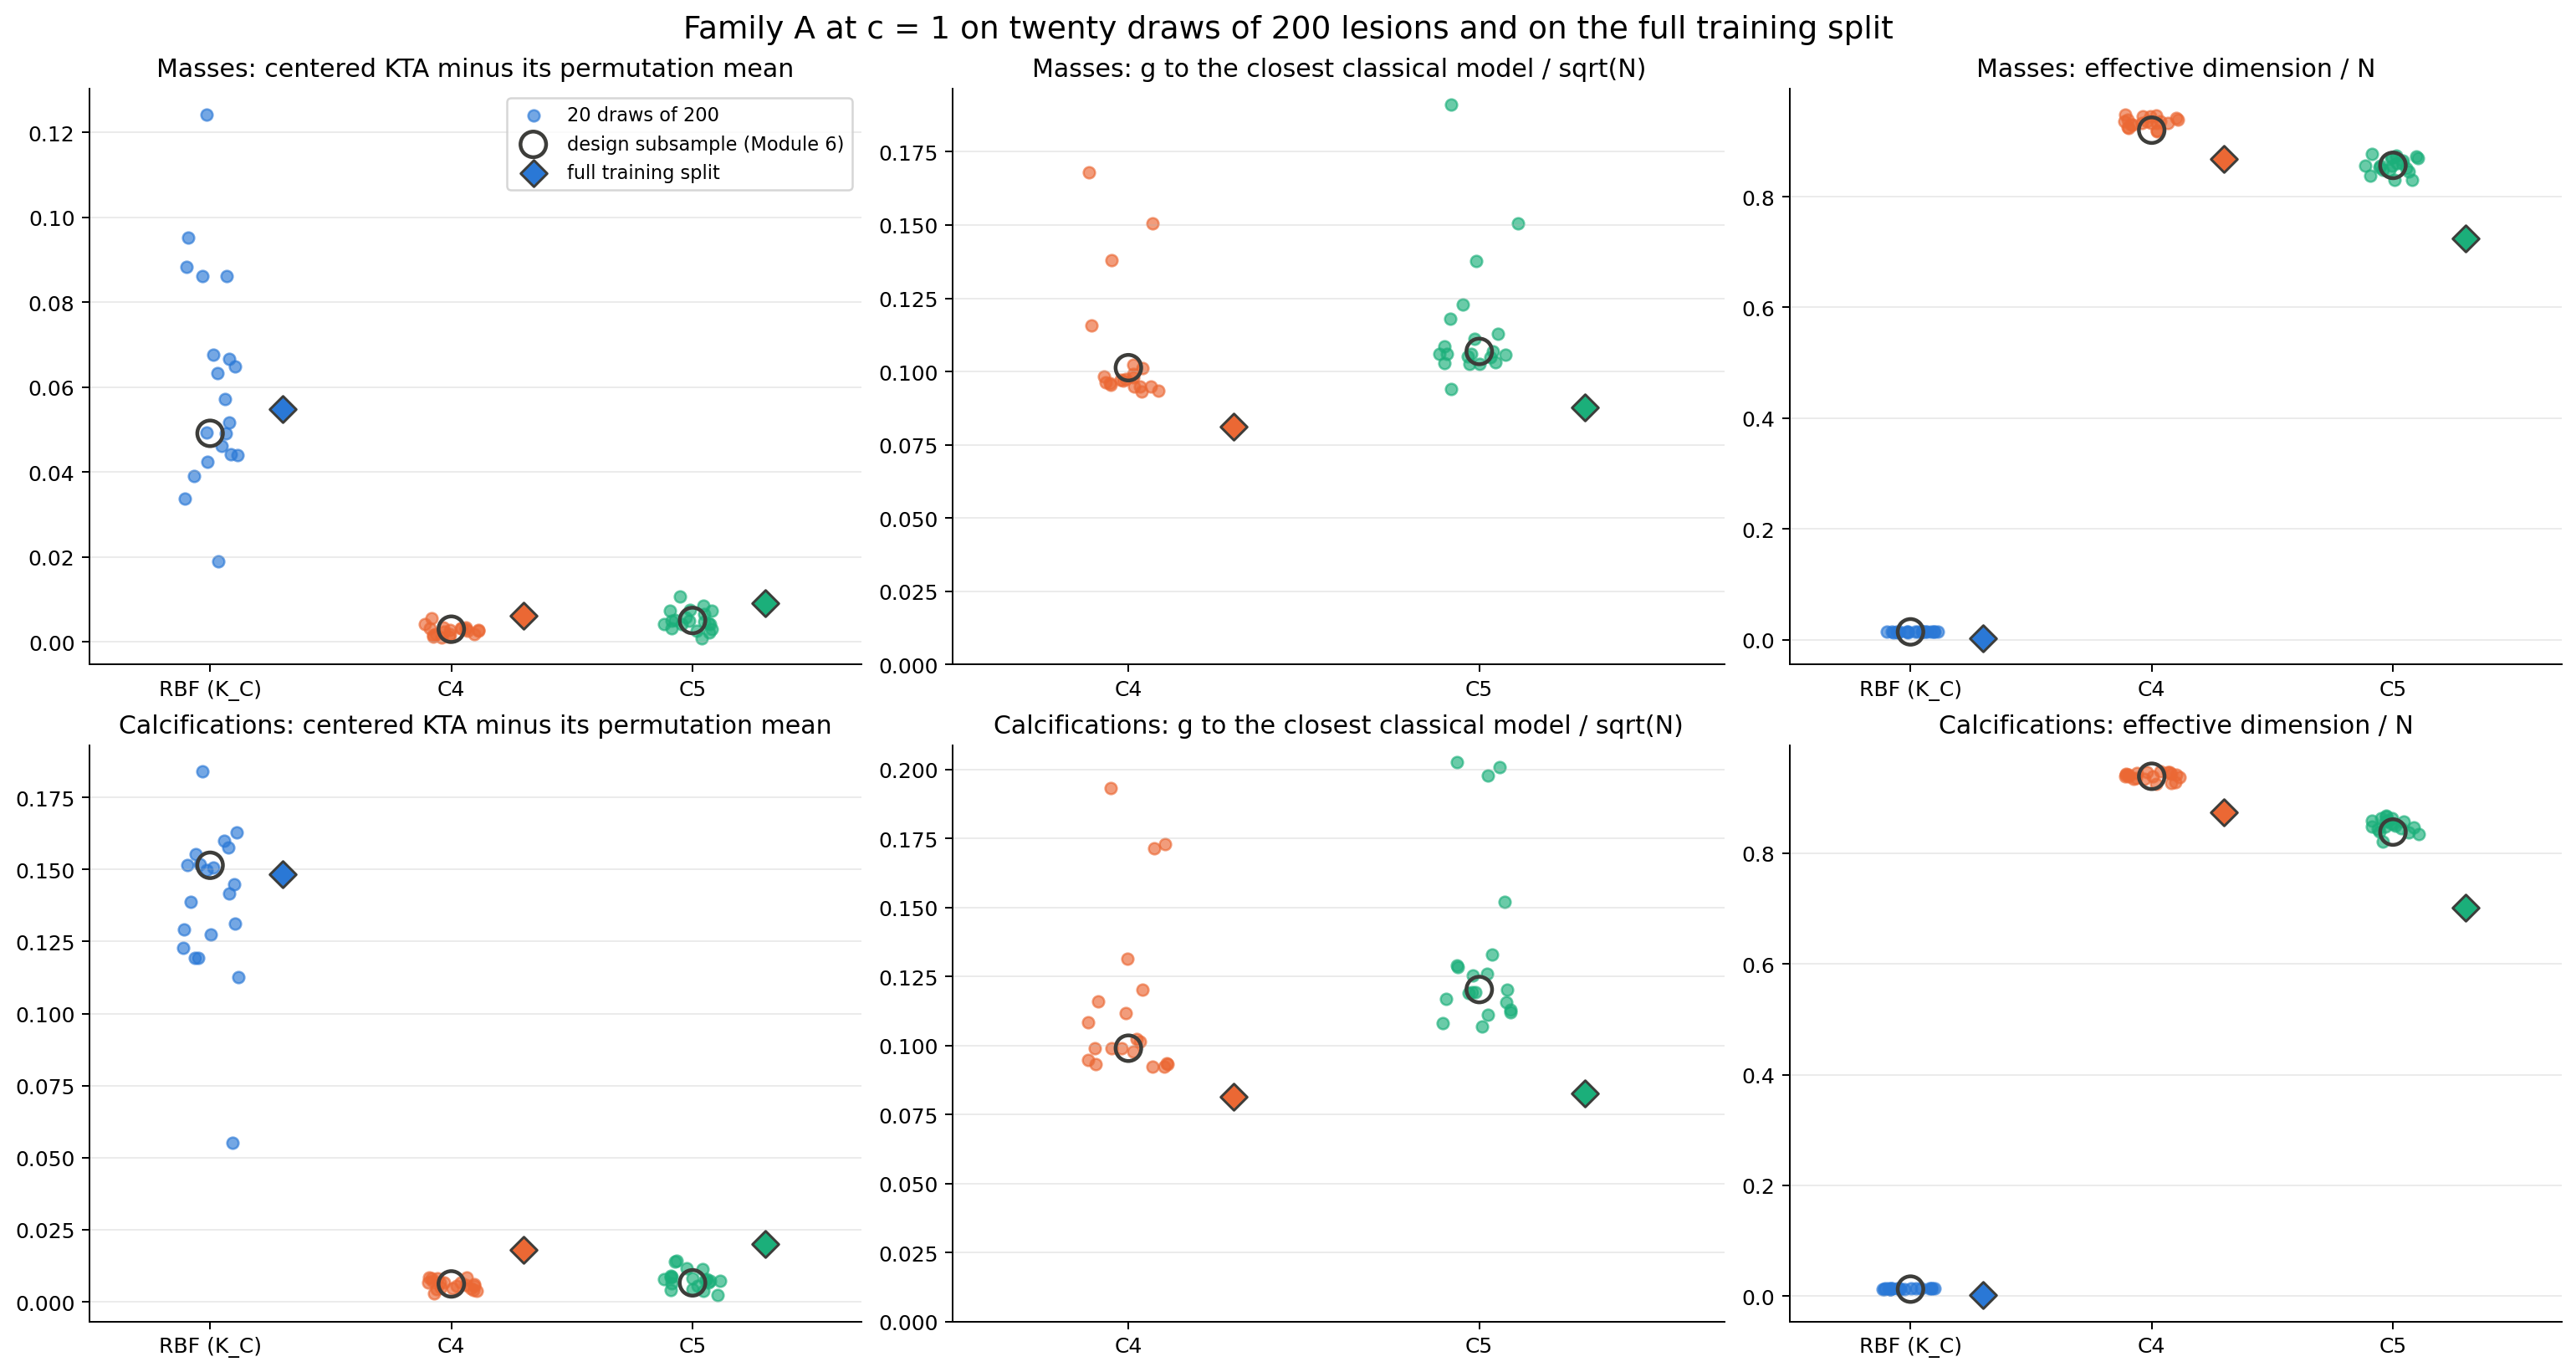
\includegraphics[width=\textwidth]{Figures/X9_sample_size.png}
% fuente: H-055; X9_familia_a.csv
\caption{Métricas de la familia de kernels a $c = 1$ en 20 submuestras de 200 lesiones (puntos), la submuestra del análisis principal (círculo) y todo el conjunto de entrenamiento (rombo).}
\label{fig:x9_sample_size}
\end{figure}

% fuente: H-036; X2_auc_pares.csv
En el análisis por pares sobre la submuestra de entrenamiento, el kernel clásico RBF obtuvo un
AUC de pares de 0.523 ($p = 0.002$) en masas y de 0.575 ($p = 0.001$) en calcificaciones. A escala $c = 1$,
C4 registró 0.510 ($p = 0.012$) en masas y 0.520 ($p = 0.021$) en calcificaciones, mientras que C5 obtuvo
0.508 ($p = 0.047$) en masas y 0.547 ($p = 0.001$) en calcificaciones. En calcificaciones, C5 superó a C4
en 0.027, aunque ambos kernels permanecieron por debajo del RBF. Al excluir los pares con fidelidad inferior
a $10^{-6}$, el AUC de pares de C5 se mantuvo en 0.510 en masas y 0.570 en calcificaciones, descartando que
la discriminación dependa de valores numéricamente irresolubles en hardware. La evolución del AUC de pares
se ilustra en la Figura~\ref{fig:x2_pair_auc_sweep}.

\begin{figure}[htbp]
\centering
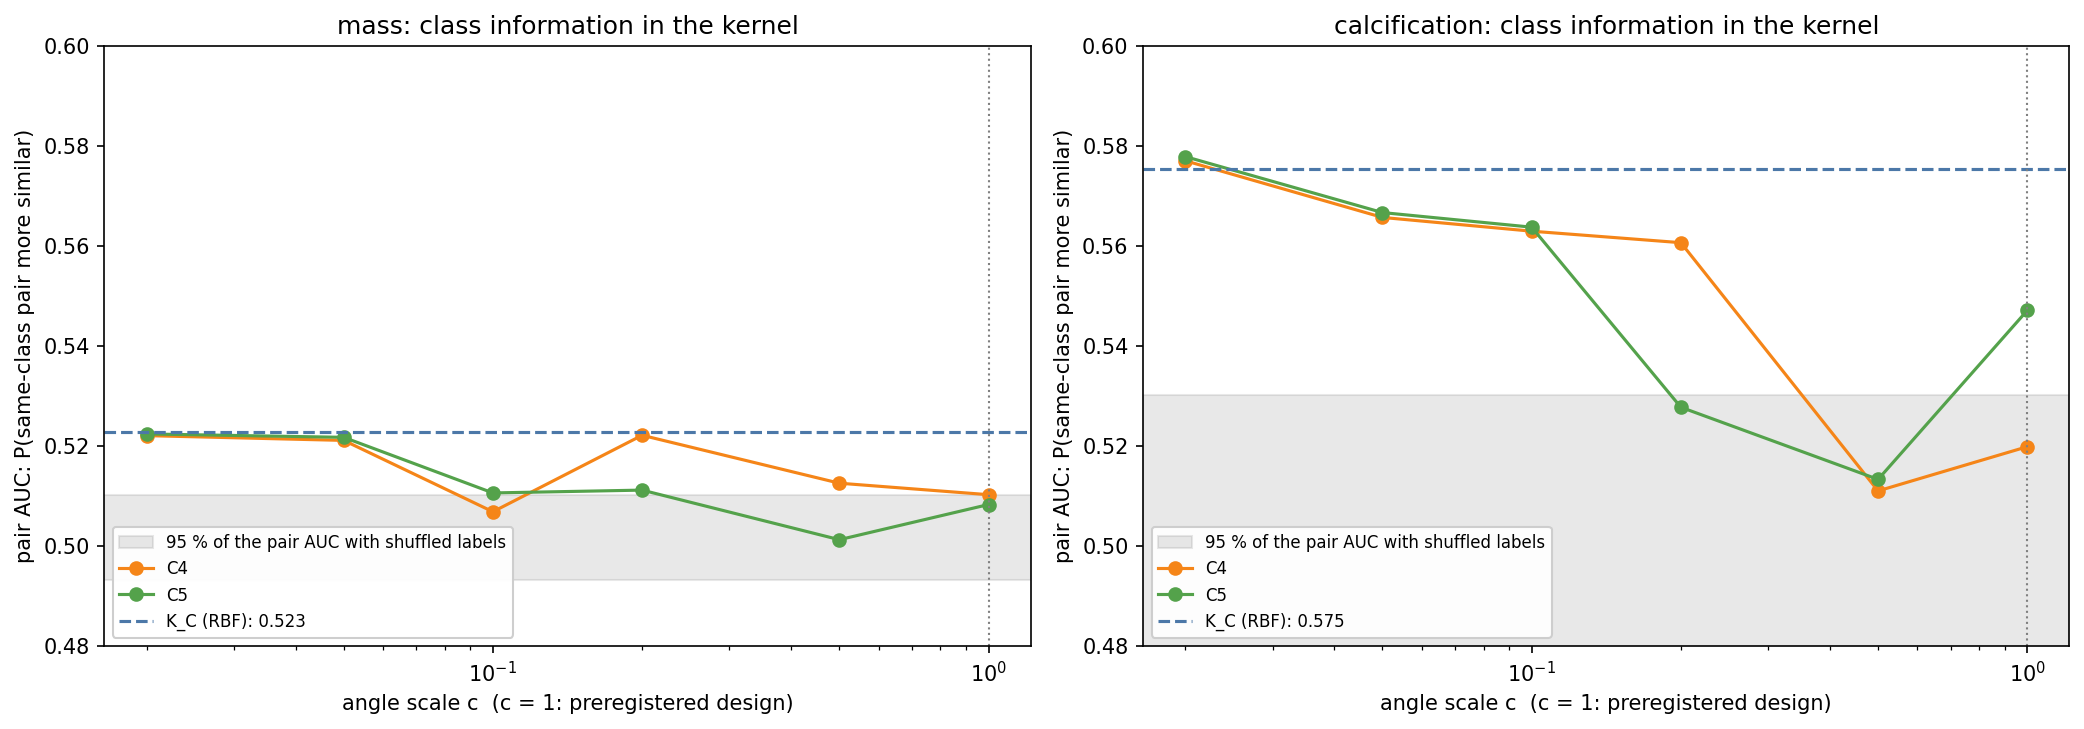
\includegraphics[width=\textwidth]{Figures/X2_pair_auc_sweep.png}
% fuente: H-036; X2_auc_pares.csv
\caption{Evolución del AUC de pares en función del factor de escala angular $c$ para kernels cuánticos y clásico.}
\label{fig:x2_pair_auc_sweep}
\end{figure}

% fuente: D-029, H-031, H-037, H-039; 8_oe6_shots_kernel.csv, 5b_concentracion_kernel.csv, 6_alineamiento_kernel.csv, 6_dimension_efectiva.csv, 6_diferencia_geometrica.csv
Al contraer los ángulos de rotación mediante el factor de escala $\mathbf{x} \to c\mathbf{x}$ con
$c \in \{1$, $0.5$, $0.2$, $0.1$, $0.05$, $0.02\}$, la concentración se reduce progresivamente: para $c = 0.02$,
la mediana fuera de la diagonal sube a 0.55 (C4) y 0.54 (C5) en masas, y a 0.59 y 0.58 en calcificaciones, el exceso de KTA alcanza
0.043 en masas y 0.143 en calcificaciones (próximo a 0.049 y 0.151 del RBF), la dimensión efectiva decae a
aproximadamente 4 y $g$ se ubica entre 2.1 y 2.5 (con un valor máximo de 3.1 en todo el barrido para C5 con $c = 0.5$).
Este incremento en alineamiento no representa información cuántica novedosa: la fase acumulada en el bloque $ZZ$
corresponde a $2\pi^2 - 2\pi c(x_i + x_j) + 2c^2 x_i x_j$, donde la fase constante es invariante y el producto
cruzado $x_i x_j$ decae con $c^2$. A escala $c = 0.02$, la correlación entre el kernel cuántico completo y una
versión idéntica que prescinde del producto entre características es de 0.99997 en masas y 0.99999 en calcificaciones.
La concentración del kernel solo se disipa cuando el término de interacción de segundo orden deja de tener efecto,
recuperando la estructura de similitud suave que un kernel clásico modela de forma directa.

% fuente: H-041; X3_comparacion_k8_k12.csv, X3_alineamiento_kernel.csv, X3_dimension_efectiva.csv, X3_diferencia_geometrica_resumen.csv
El experimento con un registro reducido a 8 qubits ($k = 8$) evaluó las ocho primeras características
de la selección con 28 bloques $ZZ$ y un circuito con 16 parámetros libres. Al reducir la dimensión, la concentración
disminuye: a $c = 1$, la mediana fuera de la diagonal asciende a 0.010 en C4 y 0.0015 en C5 para masas, y a 0.008 en C4
y 0.0008 en C5 para calcificaciones; la dimensión efectiva se reduce a 140 en C4 y 103 en C5 para masas, y a 170 en C4
y 131 en C5 para calcificaciones; y el exceso de KTA se incrementa entre 1.7 y 4.6 veces (0.012 en C4 y 0.023 en C5 para masas;
0.011 en C4 y 0.024 en C5 para calcificaciones), manteniéndose por debajo del RBF (0.049 y 0.150). La diferencia
geométrica mínima $g$ se ubicó en 2.40 en C4 y 3.23 en C5 para masas, y en 1.71 en C4 y 2.16 en C5 para calcificaciones,
muy por debajo de $\sqrt{N} = 14.1$. En las representaciones vectoriales sobre el entrenamiento completo, la condición
clásica C1 mantuvo la ventaja en la razón de Fisher: 0.37 frente a 0.09 (C4) y 0.17 (C5) en masas; y 0.98 frente a 0.29 (C4)
y 0.37 (C5) en calcificaciones. La síntesis comparativa se presenta en la Tabla~\ref{tab:comparacion_k8_k12} y la
Figura~\ref{fig:x3_kernel_metrics_k8_k12}.

% fuente: H-041; X3_comparacion_k8_k12.csv
\begin{table}[htbp]
\centering
\small
\caption{Comparación de métricas de separabilidad entre las configuraciones con $k = 12$ y $k = 8$ qubits ($c = 1$, submuestra de 200 lesiones por subconjunto).}
\label{tab:comparacion_k8_k12}
\begin{adjustbox}{max width=\linewidth}
\begin{tabular}{l r r r r}
\toprule
Métrica & Masas, $k = 12$ & Masas, $k = 8$ & Calcif., $k = 12$ & Calcif., $k = 8$ \\
\midrule
Mediana del kernel (C4 / C5) & 0.002 / 0.00003 & 0.010 / 0.0015 & 0.003 / 0.00003 & 0.008 / 0.0008 \\
Dimensión efectiva (C4 / C5 de 200) & 184.0 / 171.3 & 139.6 / 103.3 & 187.7 / 167.6 & 169.7 / 131.0 \\
Exceso de KTA (C4 / C5) & 0.003 / 0.005 & 0.012 / 0.023 & 0.006 / 0.007 & 0.011 / 0.024 \\
Exceso de KTA del RBF & 0.049 & 0.049 & 0.151 & 0.150 \\
$g$ mínima (C4 / C5; $\sqrt{N} \approx 14.1$) & 1.43 / 1.51 & 2.40 / 3.23 & 1.40 / 1.70 & 1.71 / 2.16 \\
Dispersión $\langle Z_i \rangle$ en todo el train (C4 / C5) & 0.058 / 0.180 & 0.099 / 0.276 & 0.048 / 0.178 & 0.076 / 0.267 \\
Fisher $J$ en todo el train (C1 / C4 / C5) & 0.45 / 0.13 / 0.21 & 0.37 / 0.09 / 0.17 & 1.06 / 0.42 / 0.31 & 0.98 / 0.29 / 0.37 \\
\bottomrule
\end{tabular}
\end{adjustbox}
\end{table}

\begin{figure}[htbp]
\centering
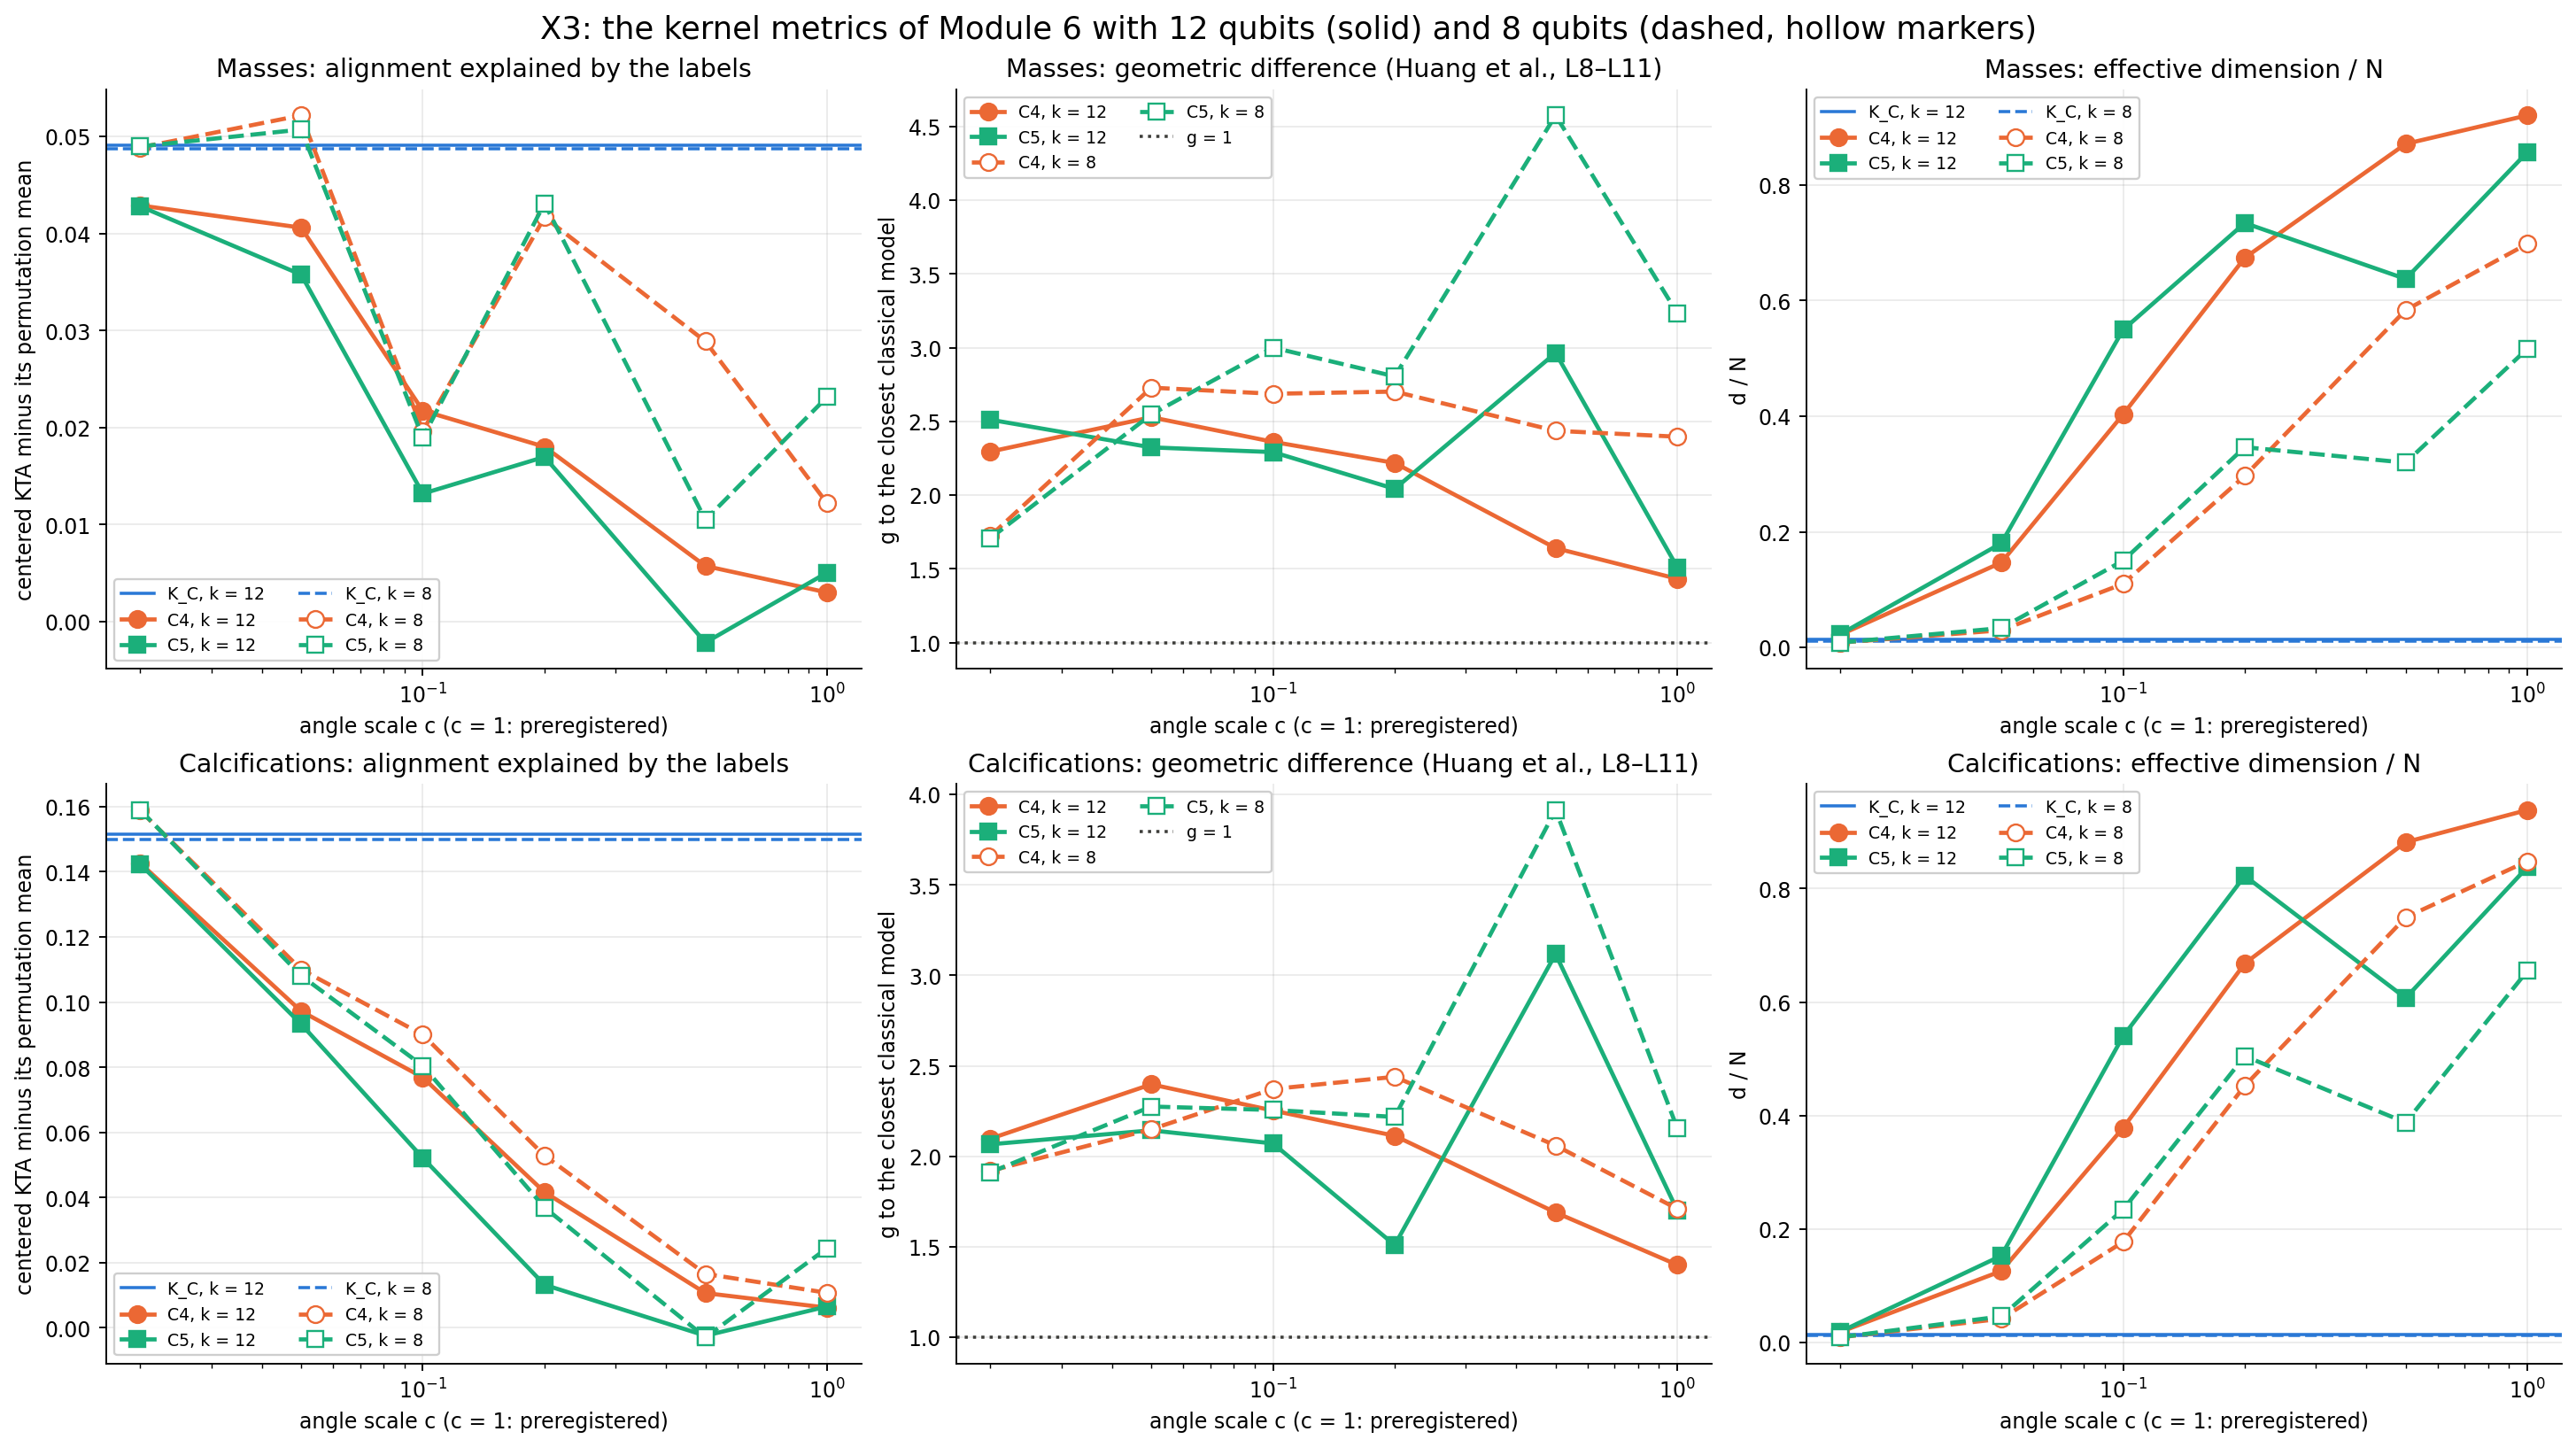
\includegraphics[width=\textwidth]{Figures/X3_kernel_metrics_k8_k12.png}
% fuente: H-041; X3_comparacion_k8_k12.csv
\caption{Comparación de métricas de separabilidad en kernels cuánticos entre configuraciones con 12 y 8 qubits.}
\label{fig:x3_kernel_metrics_k8_k12}
\end{figure}

% fuente: H-039
En conjunto, estos hallazgos proporcionan respuesta al objetivo específico OE-3: bajo la configuración
metodológica predefinida ($k = 12$, $c = 1$), las transformaciones cuánticas evaluadas no muestran una
separabilidad geométrica superior a la obtenida mediante representaciones y kernels clásicos, ni en la formulación
basada en fidelidades ni en la basada en valores esperados. Esta evidencia empírica describe la viabilidad y las
propiedades de separabilidad del espacio de estados cuánticos generado en el contexto del problema radiómico abordado.
